%%%%%%%%%%%%%%%%%%%%%%%%%%%%%%%%%%%%%%%%%
% Beamer Presentation
% LaTeX Template
% Version 2.0 (March 8, 2022)
%
% This template originates from:
% https://www.LaTeXTemplates.com
%
% Author:
% Vel (vel@latextemplates.com)
%
% License:
% CC BY-NC-SA 4.0 (https://creativecommons.org/licenses/by-nc-sa/4.0/)
%
%%%%%%%%%%%%%%%%%%%%%%%%%%%%%%%%%%%%%%%%%

%----------------------------------------------------------------------------------------
%	PACKAGES AND OTHER DOCUMENT CONFIGURATIONS
%----------------------------------------------------------------------------------------

\documentclass[
	11pt, % Set the default font size, options include: 8pt, 9pt, 10pt, 11pt, 12pt, 14pt, 17pt, 20pt
	%t, % Uncomment to vertically align all slide content to the top of the slide, rather than the default centered
	aspectratio=169, % Uncomment to set the aspect ratio to a 16:9 ratio which matches the aspect ratio of 1080p and 4K screens and projectors
]{beamer}

\graphicspath{{Images/}{./}} % Specifies where to look for included images (trailing slash required)

\usepackage{booktabs} % Allows the use of \toprule, \midrule and \bottomrule for better rules in tables

%----------------------------------------------------------------------------------------
%	SELECT LAYOUT THEME
%----------------------------------------------------------------------------------------

% Beamer comes with a number of default layout themes which change the colors and layouts of slides. Below is a list of all themes available, uncomment each in turn to see what they look like.

%\usetheme{default}
%\usetheme{AnnArbor}
%\usetheme{Antibes}
%\usetheme{Bergen}
%\usetheme{Berkeley}
%\usetheme{Berlin}
%\usetheme{Boadilla}
%\usetheme{CambridgeUS}
%\usetheme{Copenhagen}
%\usetheme{Darmstadt}
%\usetheme{Dresden}
%\usetheme{Frankfurt}
%\usetheme{Goettingen}
%\usetheme{Hannover}
%\usetheme{Ilmenau}
%\usetheme{JuanLesPins}
%\usetheme{Luebeck}
\usetheme{Madrid}
%\usetheme{Malmoe}
%\usetheme{Marburg}
%\usetheme{Montpellier}
%\usetheme{PaloAlto}
%\usetheme{Pittsburgh}
%\usetheme{Rochester}
%\usetheme{Singapore}
%\usetheme{Szeged}
%\usetheme{Warsaw}

%----------------------------------------------------------------------------------------
%	SELECT COLOR THEME
%----------------------------------------------------------------------------------------

% Beamer comes with a number of color themes that can be applied to any layout theme to change its colors. Uncomment each of these in turn to see how they change the colors of your selected layout theme.

%\usecolortheme{albatross}
%\usecolortheme{beaver}
%\usecolortheme{beetle}
%\usecolortheme{crane}
%\usecolortheme{dolphin}
%\usecolortheme{dove}
%\usecolortheme{fly}
%\usecolortheme{lily}
%\usecolortheme{monarca}
%\usecolortheme{seagull}
%\usecolortheme{seahorse}
%\usecolortheme{spruce}
%\usecolortheme{whale}
%\usecolortheme{wolverine}

%----------------------------------------------------------------------------------------
%	SELECT FONT THEME & FONTS
%----------------------------------------------------------------------------------------

% Beamer comes with several font themes to easily change the fonts used in various parts of the presentation. Review the comments beside each one to decide if you would like to use it. Note that additional options can be specified for several of these font themes, consult the beamer documentation for more information.

\usefonttheme{default} % Typeset using the default sans serif font
%\usefonttheme{serif} % Typeset using the default serif font (make sure a sans font isn't being set as the default font if you use this option!)
%\usefonttheme{structurebold} % Typeset important structure text (titles, headlines, footlines, sidebar, etc) in bold
%\usefonttheme{structureitalicserif} % Typeset important structure text (titles, headlines, footlines, sidebar, etc) in italic serif
%\usefonttheme{structuresmallcapsserif} % Typeset important structure text (titles, headlines, footlines, sidebar, etc) in small caps serif

%------------------------------------------------

%\usepackage{mathptmx} % Use the Times font for serif text
\usepackage{palatino} % Use the Palatino font for serif text

%\usepackage{helvet} % Use the Helvetica font for sans serif text
\usepackage[default]{opensans} % Use the Open Sans font for sans serif text
%\usepackage[default]{FiraSans} % Use the Fira Sans font for sans serif text
%\usepackage[default]{lato} % Use the Lato font for sans serif text
\usepackage{filecontents} % used for reference
\usepackage[style=numeric, sorting=none, backend=biber]{biblatex} % used for reference
% \usepackage[skip=1ex]{caption}
% \usepackage{subcaption}

%----------------------------------------------------------------------------------------
%	REFERENCE
%----------------------------------------------------------------------------------------

% \addbibresource{myreference.bib}

%----------------------------------------------------------------------------------------
%	SELECT INNER THEME
%----------------------------------------------------------------------------------------

% Inner themes change the styling of internal slide elements, for example: bullet points, blocks, bibliography entries, title pages, theorems, etc. Uncomment each theme in turn to see what changes it makes to your presentation.

%\useinnertheme{default}
\useinnertheme{circles}
%\useinnertheme{rectangles}
%\useinnertheme{rounded}
%\useinnertheme{inmargin}

%----------------------------------------------------------------------------------------
%	SELECT OUTER THEME
%----------------------------------------------------------------------------------------

% Outer themes change the overall layout of slides, such as: header and footer lines, sidebars and slide titles. Uncomment each theme in turn to see what changes it makes to your presentation.

%\useoutertheme{default}
%\useoutertheme{infolines}
%\useoutertheme{miniframes}
%\useoutertheme{smoothbars}
%\useoutertheme{sidebar}
%\useoutertheme{split}
%\useoutertheme{shadow}
%\useoutertheme{tree}
%\useoutertheme{smoothtree}

%\setbeamertemplate{footline} % Uncomment this line to remove the footer line in all slides
%\setbeamertemplate{footline}[page number] % Uncomment this line to replace the footer line in all slides with a simple slide count

\setbeamertemplate{navigation symbols}{} % Uncomment this line to remove the navigation symbols from the bottom of all slides
\setbeamertemplate{caption}[numbered] % numbering the figure in preentation

%----------------------------------------------------------------------------------------
%	MACRO
%----------------------------------------------------------------------------------------

\newcommand\meetingdatecompact{Meeting 11/29}
\newcommand\meetingdate{November 29, 2023}

%----------------------------------------------------------------------------------------
%	PRESENTATION INFORMATION
%----------------------------------------------------------------------------------------

\title[\meetingdatecompact]{Image Processing Prog\#3 HDR Imaging \\ \meetingdatecompact} % The short title in the optional parameter appears at the bottom of every slide, the full title in the main parameter is only on the title page

% \subtitle{Optional Subtitle} % Presentation subtitle, remove this command if a subtitle isn't required

\author[Bo Han, Chen]{Bo Han, Chen} % Presenter name(s), the optional parameter can contain a shortened version to appear on the bottom of every slide, while the main parameter will appear on the title slide

\institute[NYCU]{National Yang Ming Chiao Tung University, Taiwan \\ \smallskip \textit{bhchen312551074.cs12@nycu.edu.tw}} % Your institution, the optional parameter can be used for the institution shorthand and will appear on the bottom of every slide after author names, while the required parameter is used on the title slide and can include your email address or additional information on separate lines

\date[\meetingdate]{\meetingdate} % Presentation date or conference/meeting name, the optional parameter can contain a shortened version to appear on the bottom of every slide, while the required parameter value is output to the title slide

%----------------------------------------------------------------------------------------

\begin{document}

%----------------------------------------------------------------------------------------
%	TITLE SLIDE
%----------------------------------------------------------------------------------------

\begin{frame}
	\titlepage % Output the title slide, automatically created using the text entered in the PRESENTATION INFORMATION block above
\end{frame}

%----------------------------------------------------------------------------------------
%	TABLE OF CONTENTS SLIDE
%----------------------------------------------------------------------------------------

% The table of contents outputs the sections and subsections that appear in your presentation, specified with the standard \section and \subsection commands. You may either display all sections and subsections on one slide with \tableofcontents, or display each section at a time on subsequent slides with \tableofcontents[pausesections]. The latter is useful if you want to step through each section and mention what you will discuss.

\begin{frame}
	\frametitle{Presentation Overview} % Slide title, remove this command for no title
	
	\tableofcontents % Output the table of contents (all sections on one slide)
	%\tableofcontents[pausesections] % Output the table of contents (break sections up across separate slides)
\end{frame}

%----------------------------------------------------------------------------------------
%	PRESENTATION BODY SLIDES
%----------------------------------------------------------------------------------------

\section{Environment}

\begin{frame}
	\frametitle{Environment}

	\begin{itemize}
		\item Windows 10 22H2
		\item Python 3.12.0
		\begin{itemize}
			\item OpenCV 4.8.1
		\end{itemize}
	\end{itemize}
\end{frame}

\section{Motivation}

\begin{frame}
	\frametitle{Motivation}

	\begin{itemize}
		\item exposure $X$ vs. pixel value $Z$
		\item unknown, nonlinear mapping $Z = f(X)$
		\item objective: recover $E$ from $Z$
		\item how: using multiple photo with different exposure
	\end{itemize}
	
	\begin{figure}
		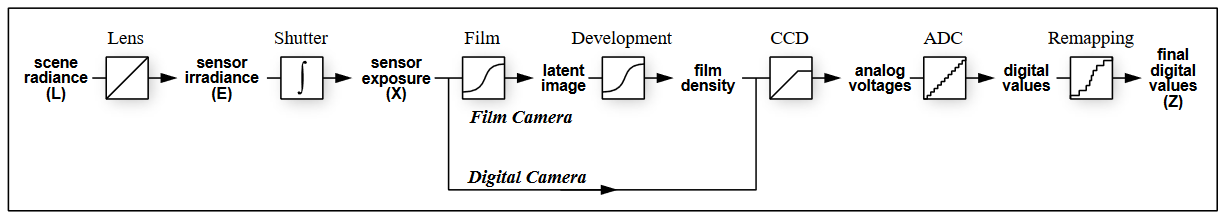
\includegraphics[width=0.9\linewidth]{./Images/camera_pipeline.png}
		\caption{Image Acquisition Pipeline}
	\end{figure}

\end{frame}

\section{Debevec's Method}
\subsection{Algorithm}

\begin{frame}
	\frametitle{Debevec's Method}
	\framesubtitle{Algorithm}

	\begin{itemize}
		\item recovering the radiance map $E_i$ from the pixel values $Z_{ij}$
		\begin{itemize} 
			\item $X = E_i \Delta t_j$
			\item $f(X) = f(E_i \Delta_j) = Z_{ij}$
			\item $g = \ln f^{-1}$
			\item $g(Z_{ij}) = \ln E_i + \ln \Delta t_j$
		\end{itemize}
		\item solving $g$ and $E_i$ with SVD
	\end{itemize}

	\begin{figure}
		$$O = \sum _{i=1}^{N} \sum_{j=1}^{P} \left[g(Z_{ij}) - \ln E_i - \ln \Delta t_j\right]^{2} 
			+ \lambda \sum_{z = Z_{min} + 1}^{Z_{max} - 1} g''(z)^{2}$$
		\caption{Objective Function}
	\end{figure}
\end{frame}

\begin{frame}
	\frametitle{Debevec's Method}
	\framesubtitle{Additional Settings}

	\begin{itemize}
		% \item $\lambda$
		% \begin{itemize}
		% 	\item determined by noise level
		% \end{itemize}
		\item $g(Z_{mid}) = 0$
		\begin{itemize}
			\item fix the curve
			\item set pixel value $Z_{mid}$ to the unit exposure
		\end{itemize}
		\item weighted function $w(Z)$
		\begin{itemize}
			\item emphasize the smoothness
			\item fitting terms toward the middle of curve
		\end{itemize}
		\item pixel value selection
		\begin{itemize}
			\item even distribution
			\item sampled from low intensity variance region
			\item how many sample value we need?
		\end{itemize}
	\end{itemize}
\end{frame}

% Further-
% more, the pixels are best sampled from regions of the image with
% low intensity variance so that radiance can be assumed to be con-
% stant across the area of the pixel, and the effect of optical blur of the
% imaging system is minimized

\begin{frame}
	\frametitle{Debevec's Method}
	\framesubtitle{Constructing \& Display HDR Radiance Map}

	\begin{itemize}
		\item reconstruct $E$ with $g$
		\begin{itemize}	
			\item by using all available exposures
		\end{itemize}
		\item display
		\begin{itemize}
			\item take logarithm
			\item linearly map to device range
		\end{itemize}
	\end{itemize}
\end{frame}

\subsection{Experiment}

\begin{frame}
	\frametitle{Experiment}
	\framesubtitle{Image}

	\begin{itemize}
		\item 14 images handheld-shot by Xiaomi 12T Pro
		\item ISO: 800
		\item Aperture: f/1.69
		\item Exposure Time: 1/1000, 1/800, 1/400, 1/250, 1/200, 1/125, 1/80, 
		1/30, 1/15, 1/8, 1/4, 1/2, 1, 2, 4
	\end{itemize}

	\begin{figure}[!htb]
		\minipage{0.32\textwidth}
		  \includegraphics[width=\linewidth]{../images/scene1/1701116928525.jpg}
		\endminipage\hfill
		\minipage{0.32\textwidth}
		  \includegraphics[width=\linewidth]{../images/scene1/1701116928549.jpg}
		\endminipage\hfill
		\minipage{0.32\textwidth}%
		  \includegraphics[width=\linewidth]{../images/scene1/1701116928563.jpg}
		\endminipage
		\caption{Test Image (Exposure Time: 1/1000, 1/30, 1/2)}
	\end{figure}
\end{frame}

\begin{frame}
	\frametitle{Experiment}
	\framesubtitle{Experiment Settings}

	\begin{itemize}
		\item pixel sampling
		\begin{itemize}
			\item 100 pixels per exposure time
		\end{itemize}
		\item parameter
		\begin{itemize}
			\item $\lambda = 10$
			\item $Z_{min} = 0, Z_{max} = 255$
		\end{itemize}
		\item display HDR image
		\begin{itemize}
			\item linear mapping
			\item tone mapping (with OpenCV)
		\end{itemize}
	\end{itemize}
\end{frame}

\begin{frame}
	\frametitle{Experiment}
	\framesubtitle{Response Curve}

	\begin{figure}
		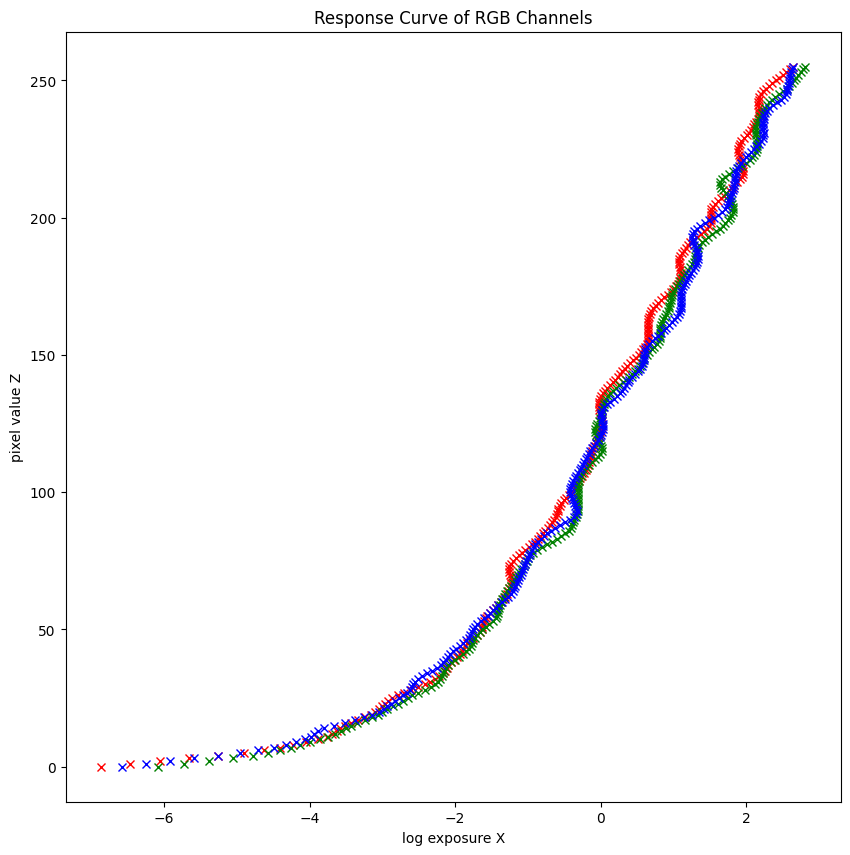
\includegraphics[width=0.4\linewidth]{./Images/response_curve.png}
		\caption{Response Curve}
	\end{figure}
\end{frame}

\begin{frame}
	\frametitle{Experiment}
	\framesubtitle{HDR Radiance Map}

	\begin{figure}
		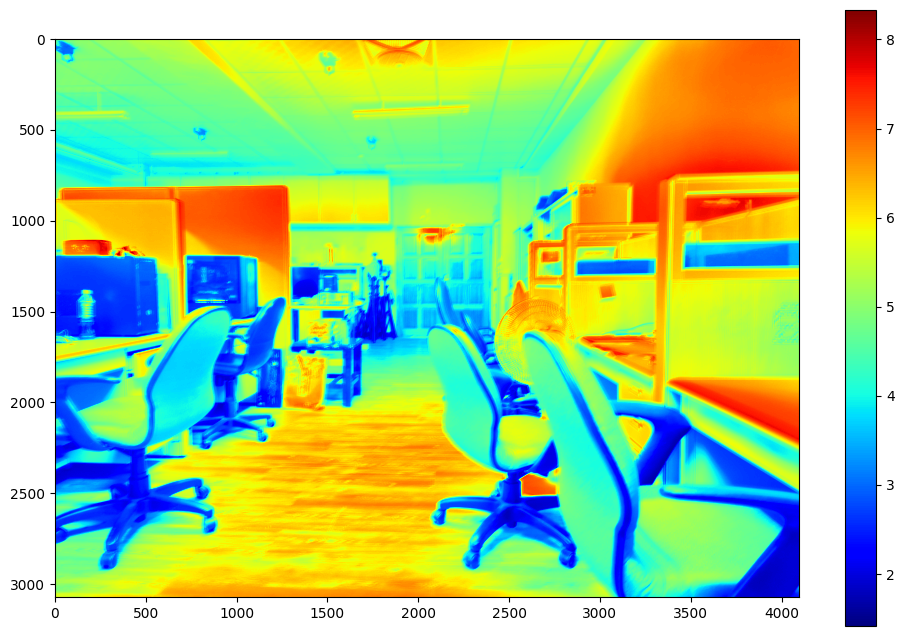
\includegraphics[width=0.55\linewidth]{./Images/hdr_radiance_map.png}
		\caption{HDR Radiance Map}
	\end{figure}
\end{frame}

\begin{frame}
	\frametitle{Experiment}
	\framesubtitle{HDR Image}

	\begin{figure}
		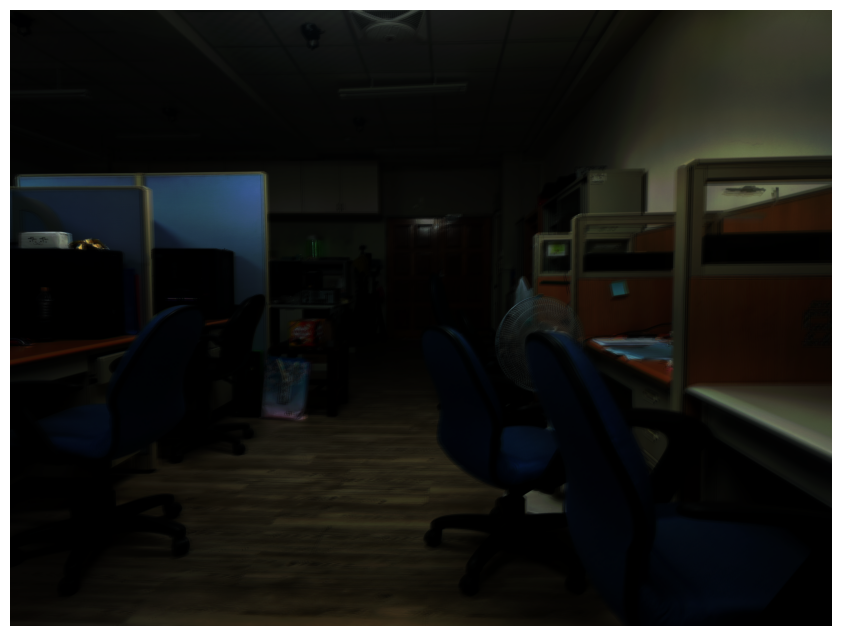
\includegraphics[width=0.45\linewidth]{./Images/hdr_linear_map.png}
		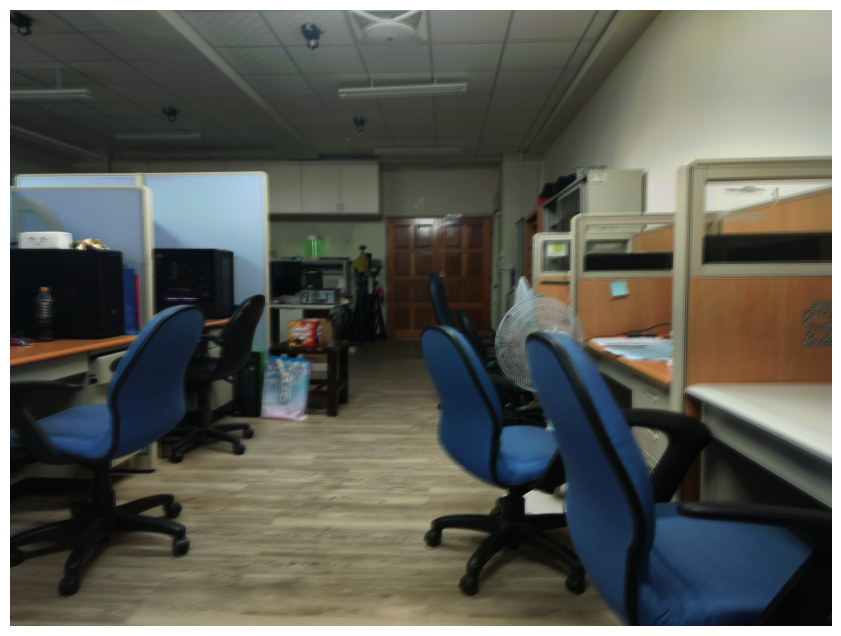
\includegraphics[width=0.45\linewidth]{./Images/hdr_tone_map.png}
		\caption{HDR Image}
	\end{figure}
\end{frame}

\section{MTB Alignment}
\subsection{Algorithm}

\begin{frame}
	\frametitle{MTB Alignment}
	\framesubtitle{Motivation}
	
	% \begin{figure}
	% 	\includegraphics[width=0.4\linewidth]{../images/scene1/1701116928545.jpg}
	% 	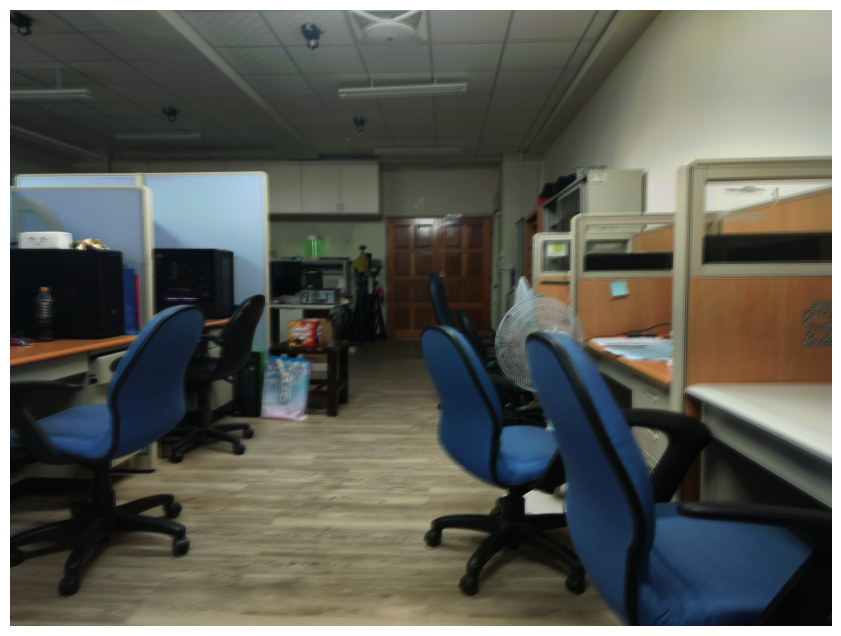
\includegraphics[width=0.4\linewidth]{./Images/hdr_tone_map.png}
	% 	\caption{Blurred HDR Image}
	% \end{figure}

	\begin{tabular}{cl}  
		\begin{tabular}{c}
			\parbox{0.4\linewidth}{
				\begin{itemize}
					\item slight camera movement during exposure
					\item blurred images
				\end{itemize}
			}
		\end{tabular}
		& \begin{tabular}{c}
			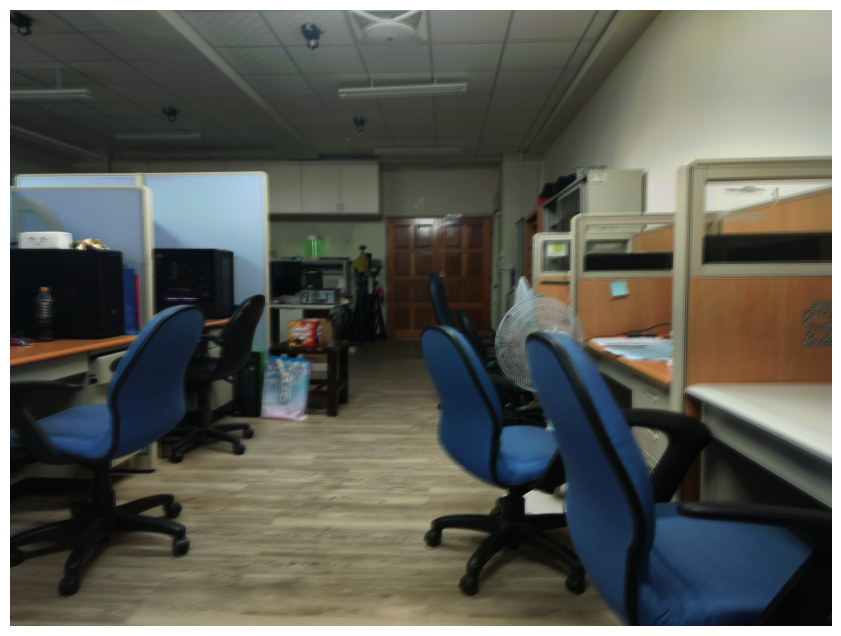
\includegraphics[width=0.5\linewidth]{./Images/hdr_tone_map.png}
		\end{tabular}  \\
 	\end{tabular}

\end{frame}

\begin{frame}
	\frametitle{MTB Alignment}
	\framesubtitle{Approaches}

	\begin{tabular}{cl}  
		\begin{tabular}{c}
			\parbox{0.44\linewidth}{
				\begin{itemize}
					\item offset relative to the reference image
					\item edge-detection
					\begin{itemize}
						\item dependent on exposure
					\end{itemize}
				\end{itemize}
			}
		\end{tabular}
		& \begin{tabular}{c}
			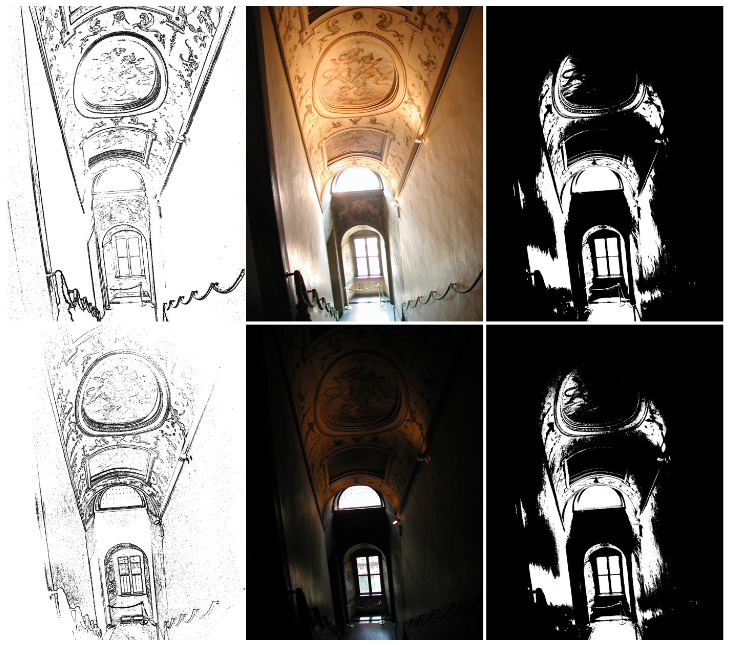
\includegraphics[width=0.5\linewidth]{./Images/mtb_example.png}
		\end{tabular}  \\
 	\end{tabular}

\end{frame}

\begin{frame}
	\frametitle{MTB Alignment}
	\framesubtitle{Median Threshold Bitmap}

	\begin{itemize}
		\item advantages
		\begin{itemize}
			\item insentive to exposure
			\item bit-manipulation routines
		\end{itemize}
		\item for exterme cases
		\begin{itemize}
			\item choosing either 17th or 83th percentile
			\item limit the maximum offset
		\end{itemize}
	\end{itemize}
\end{frame}

% \begin{frame}
% 	\frametitle{MTB Alignment}
% 	\framesubtitle{Image Pyramid}

% 	\begin{figure}
% 		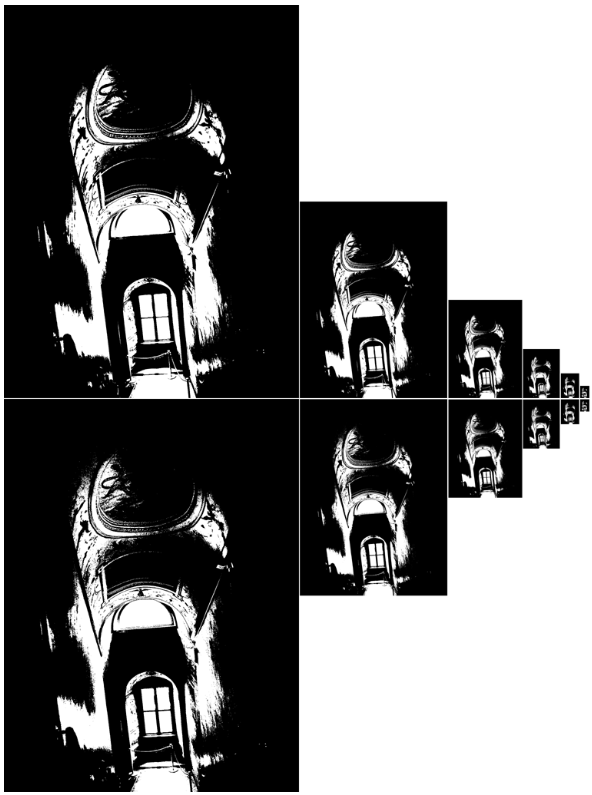
\includegraphics[width=0.3\linewidth]{./Images/image_pyramid.png}
% 		\caption{Image Pyramid}
% 	\end{figure}
% \end{frame}

\begin{frame}
	\frametitle{MTB Alignment}
	\framesubtitle{Image Pyramid}

	\begin{tabular}{cl}  
		\begin{tabular}{l}
			\parbox{0.5\linewidth}{
				\begin{itemize}
					\item compare to the reference image
					\item for each dimension ($x, y$) and resolution
					\begin{itemize}
						\item $\Delta x_1 = \pm(1, 0)$
						\item $\Delta x_2 = 2 \Delta x_1 \pm(1, 0)$
						\item ...
					\end{itemize}
				\end{itemize}
			}
		\end{tabular}
		& \begin{tabular}{c}
			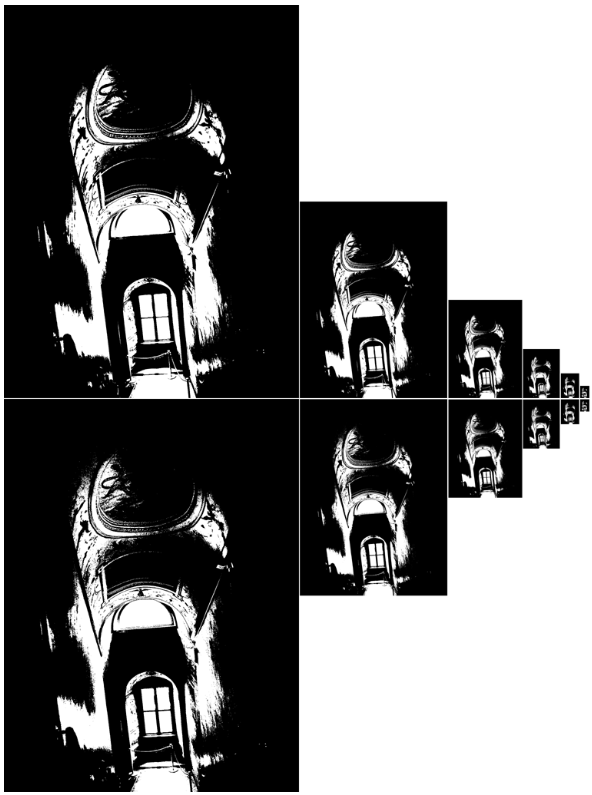
\includegraphics[width=0.3\linewidth]{./Images/image_pyramid.png}
		\end{tabular}  \\
 	\end{tabular}

\end{frame}

\begin{frame}
	\frametitle{MTB Alignment}
	\framesubtitle{Threshold Noise}

	\begin{tabular}{cl}  
		\begin{tabular}{c}
			\parbox{0.5\linewidth}{
				\begin{itemize}
					\item too many pixel value near the median cause noise in MTB
					\item makes XOR difference unstable
					\item solution
					\begin{itemize}
						\item exclude pixels from specified distances of the threshold
						\item AND with both exclusion map
					\end{itemize}
				\end{itemize}
			}
		\end{tabular}
		& \begin{tabular}{c}
			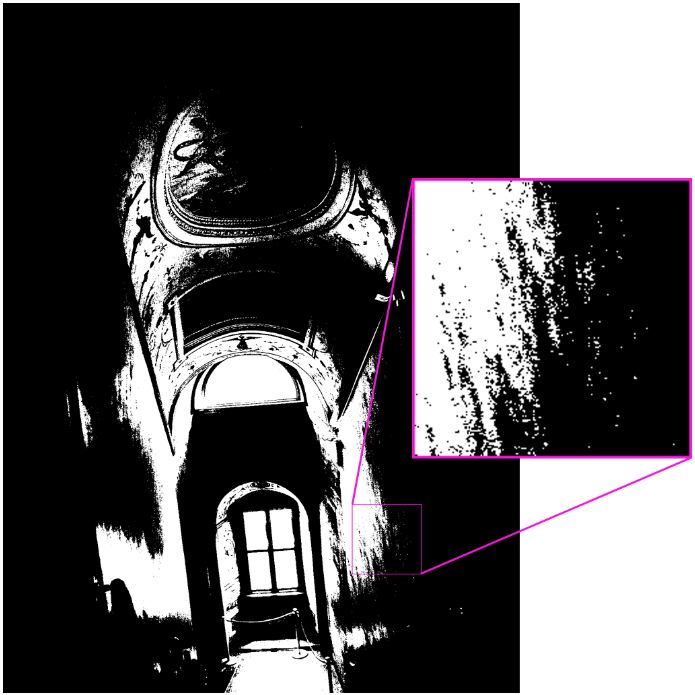
\includegraphics[width=0.4\linewidth]{./Images/mtb_noise.png}
		\end{tabular}  \\
 	\end{tabular}
\end{frame}

\subsection{Experiment}

\begin{frame}
	\frametitle{Experiment}
	\framesubtitle{Experiment Settings}

	\begin{itemize}
		\item same image set
		\item parameter
		\begin{itemize}
			\item grayscale traslation: $\frac{54 \cdot R + 183 \cdot G + 19 \cdot B}{256}$
			\item maximum offset: 4
			\item noise exclusion distance: $\pm 4$
		\end{itemize}
	\end{itemize}
\end{frame}

\begin{frame}
	\frametitle{Experiment}
	\framesubtitle{Grayscale \& MTB}

	\begin{figure}
		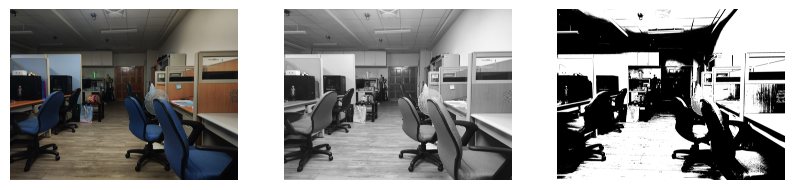
\includegraphics[width=\linewidth]{./Images/mtb_image.png}
		\caption{Original, Grayscale \& MTB}
	\end{figure}
\end{frame}

\begin{frame}
	\frametitle{Experiment}
	\framesubtitle{Noise Threshold}

	\begin{figure}
		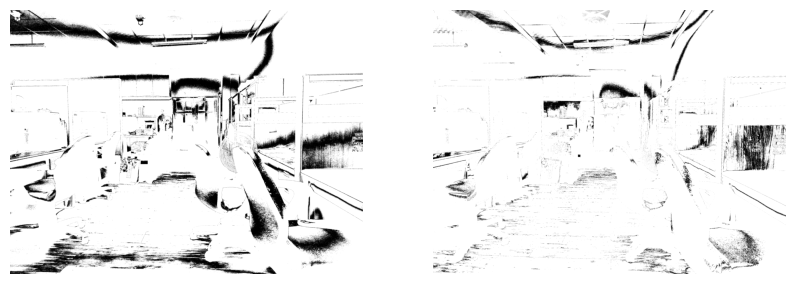
\includegraphics[width=\linewidth]{./Images/mtb_exclusion_map.png}
		\caption{Exclusion Map}
	\end{figure}
\end{frame}

\begin{frame}
	\frametitle{Experiment}
	\framesubtitle{XOR Operation}

	\begin{figure}
		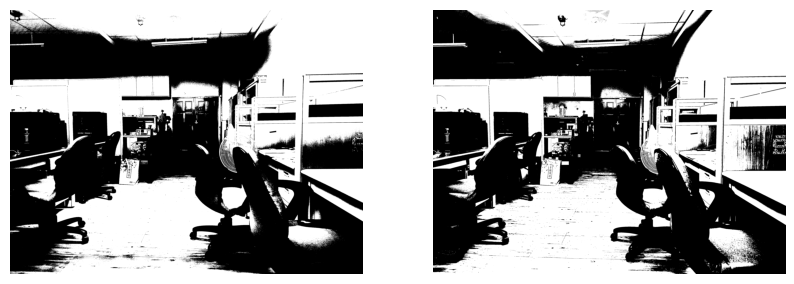
\includegraphics[width=\linewidth]{./Images/mtb_diff_operand.png}
		\caption{MTB of Ref Image and Unaligned Image}
	\end{figure}
\end{frame}

\begin{frame}
	\frametitle{Experiment}
	\framesubtitle{XOR Operation}

	\begin{figure}
		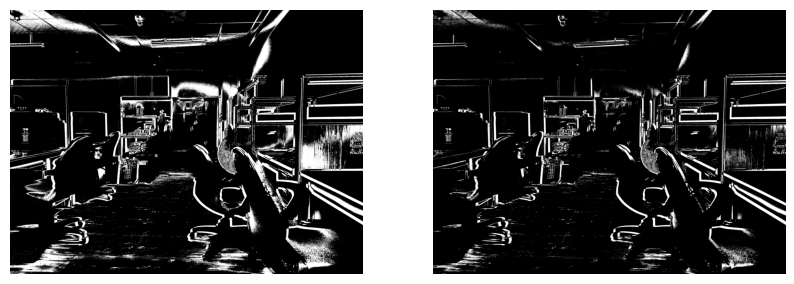
\includegraphics[width=\linewidth]{./Images/mtb_diff.png}
		\caption{XOR Difference (with \& without noise exclusion)}
	\end{figure}
\end{frame}

\section{Discussion}

\begin{frame}
	\frametitle{Discussion \& Future Work}

	\begin{tabular}{cl}  
		\begin{tabular}{c}
			\parbox{0.4\linewidth}{
				\begin{itemize}
					\item Debevec's Method
					\begin{itemize}
						\item parameter tuning
						% such as $\lambda$, weighted function and sampling method
						\item issues with color image
						\item limitation related to pixel and exposure value distribution
					\end{itemize}
					\item MTB Alignment
					\begin{itemize}
						\item selection of reference image
					\end{itemize}
					\item improving image selection
					\item compare with deep learning-based method
				\end{itemize}
			}
		\end{tabular}
		& \begin{tabular}{c}
			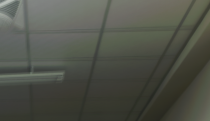
\includegraphics[width=0.5\linewidth]{./Images/hdr_color_issue.png}
		\end{tabular}  \\
 	\end{tabular}

\end{frame}

\section{References}

\begin{frame}
	\frametitle{References}
	
	\begin{itemize}
		\item Debevec, Paul E., and Jitendra Malik. 
		"Recovering high dynamic range radiance maps from photographs."
		\item Ward, Greg. "Fast, robust image registration for compositing 
		high dynamic range photographs from hand-held exposures."
		% \item Eilertsen, Gabriel, et al. "HDR image reconstruction from a 
		% single exposure using deep CNNs."
	\end{itemize}
\end{frame}

%------------------------------------------------

% \section{References}

% \begin{frame}
% 	\frametitle{References}

% 	\printbibliography
% \end{frame}

%----------------------------------------------------------------------------------------
%	CLOSING SLIDE
%----------------------------------------------------------------------------------------

\section{Q \& A}

\begin{frame}
    \frametitle{Q \& A}
	\begin{center}
		{\Huge Thanks for Listening}
		
		\bigskip\bigskip % Vertical whitespace
		
		{\LARGE Q \& A}

		% \bigskip\bigskip
		% Contact Me: b083040012@g-mail.nsysu.edu.tw
	\end{center}
\end{frame}

%----------------------------------------------------------------------------------------

\end{document} 